% !TeX root = ../main.tex

\newlecture[Mean-Variance Portfolio Theory][Nov 5, 2026]

\header{Motivation}
We want a theory of \dbb{single period random cash flows}. Random quantities are characterized by their probability distributions, but these are hard to work with. Instead, we characterize a single period investment by its \rb{expected return} and its \rb{standard deviation}, which are easier to work with.
\keypoint{Think of this as a \rb{reward/risk} description: expected return $=$ reward, standard deviation $=$ risk.}

\header{Basic Probability}
\begin{definition}[\rb{Discrete Random Variable}]
    A variable $X$ that can take on the values $x_1, x_2, \dots, x_n$ with probabilities $p_1, p_2, \dots, p_n$:
    \[X = \begin{cases}
        x_1 & \text{w.p. } p_1\\
        x_2 & \text{w.p. } p_2\\
        \ \vdots & \quad\vdots\\
        x_n & \text{w.p. } p_n
    \end{cases} \qquad \text{where } p_i \geq 0 \text{ and } \sum_{i=1}^{n}p_i = 1\]
    Writing the probabilities $p_i$ as a function of $x_i$ gives the \rb{probability mass function} (PMF).
\end{definition}

\begin{center}
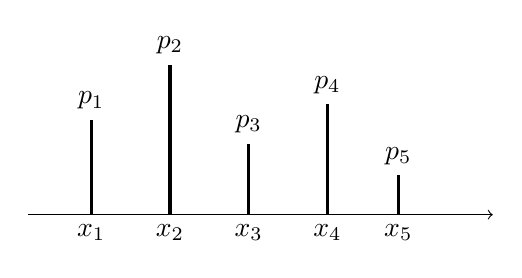
\begin{tikzpicture}
    \draw[->] (-0.3,0) -- (5.6,0);
    \foreach \x/\h/\i in {0.5/1.2/1, 1.5/1.9/2, 2.5/0.9/3, 3.5/1.4/4, 4.4/0.5/5} {
        \draw[very thick] (\x,0) -- (\x,\h) node[above] {$p_\i$};
        \node[below] at (\x,0) {$x_\i$};
    }
\end{tikzpicture}
\end{center}

\begin{definition}[\rb{Expectation}]
    \[\boxed{\overline{X} = E[X] = \sum_{i=1}^{n}x_ip_i}\]
\end{definition}
Properties:
\begin{itemize}
    \item \b{Certain value}: if $y$ is known (not random), then $E[y] = y$.
    \item \b{Linearity}: for random variables $X, Y$ and constants $a, b$: $E[aX + bY] = aE[X] + bE[Y]$.
    \item \b{Non-negativity}: if $X$ only takes positive values, then $E[X] > 0$.
\end{itemize}

\begin{definition}[\rb{Variance and Standard Deviation}]
    \[\boxed{\operatorname{Var}(X) = \sigma_X^2 = E\left[(X - \overline{X})^2\right] = E[X^2] - \overline{X}^2}\qquad \boxed{\sigma_X = \sqrt{\operatorname{Var}(X)}}\]
    The standard deviation has the \dbb{same units as $X$} and measures the spread of a random variable around its mean.
\end{definition}

\begin{example}[Roll of a Die]
    $X = 1, 2, \dots, 6$, each w.p.\ $\frac{1}{6}$.
    \begin{center}
    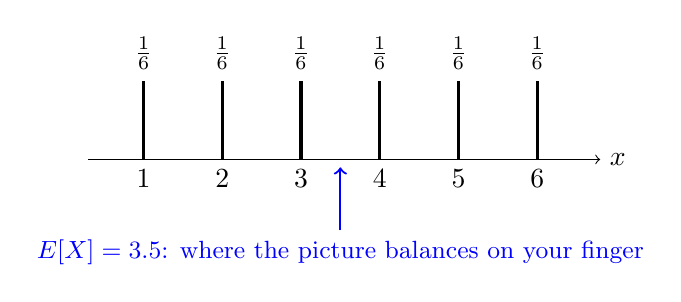
\begin{tikzpicture}
        \draw[->] (0.3,0) -- (6.8,0) node[right] {$x$};
        \foreach \x in {1,...,6} {
            \draw[very thick] (\x,0) -- (\x,1) node[above] {$\frac{1}{6}$};
            \node[below] at (\x,0) {\x};
        }
        \draw[->, thick, blue] (3.5,-0.9) -- (3.5,-0.1);
        \node[blue, below] at (3.5,-0.9) {\small $E[X] = 3.5$: where the picture balances on your finger};
    \end{tikzpicture}
    \end{center}
    \[E[X] = \sum_{i=1}^{6}x_ip_i = 1\cdot\tfrac{1}{6} + 2\cdot\tfrac{1}{6} + \cdots + 6\cdot\tfrac{1}{6} = \sum_{i=1}^{6}\frac{i}{6} = 3.5\]
    \[\operatorname{Var}(X) = \tfrac{1}{6}(1-3.5)^2 + \tfrac{1}{6}(2-3.5)^2 + \cdots + \tfrac{1}{6}(6-3.5)^2 = 2.92\]
    Check with the shortcut: $E[X^2] - \overline{X}^2 = \frac{91}{6} - 3.5^2 = 2.92$.
\end{example}

\header{Multiple Random Variables}
Let $X_1$ and $X_2$ be two random variables. A \rb{joint probability mass function} assigns to each outcome $(X_1, X_2) = (x_i^1, x_j^2)$ a probability $p_{ij}$.

$X_1$ and $X_2$ are \rb{independent} if the outcome of one does not depend on, or affect, the outcome of the other. More specifically:
\[\Pr(X_1 = x_i^1, X_2 = x_j^2) = \Pr(X_1 = x_i^1)\Pr(X_2 = x_j^2) \quad \Rightarrow \quad E[X_1X_2] = E[X_1]E[X_2]\]

\begin{definition}[\rb{Covariance}]
    \[\boxed{\sigma_{12} = \operatorname{Cov}(X_1, X_2) = E\left[(X_1 - \overline{X}_1)(X_2 - \overline{X}_2)\right] = E[X_1X_2] - \overline{X}_1\overline{X}_2}\]
    Covariance measures the \dbb{dependence} between random variables.
    \begin{itemize}
        \item If $X_1$ and $X_2$ are independent, then $\operatorname{Cov}(X_1, X_2) = 0$.
        \item The covariance of $X_1$ with itself is $\operatorname{Cov}(X_1, X_1) = \operatorname{Var}(X_1)$, i.e.\ $\sigma_{11} = \sigma_1^2$.
    \end{itemize}
\end{definition}

We say $X_1$ and $X_2$ are
\begin{center}
\begin{tabular}{rl}
    \rb{uncorrelated} & if $\sigma_{12} = 0$\\
    \rb{positively correlated} & if $\sigma_{12} > 0$\\
    \rb{negatively correlated} & if $\sigma_{12} < 0$
\end{tabular}
\end{center}
\b{Intuition}: positive correlation means that when $X_1$ is above its mean, $X_2$ is likely to also be above its mean, i.e.\ they ``tend to move in the same direction''. Negative correlation means they tend to move in opposite directions.

\begin{definition}[\rb{Correlation Coefficient}]
    \[\boxed{\rho_{12} = \frac{\sigma_{12}}{\sigma_1\sigma_2}}\]
    Since the covariance satisfies $|\sigma_{12}| \leq \sigma_1\sigma_2$, this guarantees $|\rho_{12}| \leq 1$.
    \begin{itemize}
        \item $\rho_{12} = 1$: \rb{perfectly correlated} ($X_2 = aX_1 + b$, $a > 0$).
        \item $\rho_{12} = -1$: \rb{perfect negative correlation} ($X_2 = aX_1 + b$, $a < 0$).
    \end{itemize}
\end{definition}

\begin{center}
\begin{tikzpicture}[scale=0.9]
    \foreach \sx/\lab/\slope in {0/{\rho = 1}/0.7, 4.5/{\rho \approx 0}/0, 9/{\rho = -1}/-0.7} {
        \begin{scope}[xshift=\sx cm]
            \draw[->] (-1.5,0) -- (1.6,0) node[right] {\small $X$};
            \draw[->] (0,-1.3) -- (0,1.4) node[above] {\small $Y$};
            \node at (0,-1.7) {$\lab$};
        \end{scope}
    }
    % rho = 1 and rho = -1: points on a line
    \foreach \x in {-1.2,-0.9,-0.6,-0.35,-0.1,0.2,0.45,0.7,0.95,1.2} {
        \fill[blue] (\x,0.7*\x) circle (1.6pt);
        \fill[blue] (9+\x,-0.7*\x) circle (1.6pt);
    }
    % rho ~ 0: scattered cloud
    \foreach \x/\y in {-1.1/0.6, -0.8/-0.7, -0.5/0.2, -0.3/-1.0, -0.1/0.9, 0.2/-0.3, 0.4/0.5, 0.6/-0.8, 0.9/0.1, 1.1/-0.4, -0.7/1.0, 0.7/0.9} {
        \fill[blue] (4.5+\x,\y) circle (1.6pt);
    }
\end{tikzpicture}
\end{center}
The slide's spreadsheet example simulates $\rho = -1$: every point lies exactly on a line of negative slope.

\header{Mean and Variance of a Sum}
By linearity of expectation:
\[E[X_1 + X_2] = E[X_1] + E[X_2], \qquad \text{more generally} \qquad \boxed{E\left[\sum_i a_iX_i\right] = \sum_i a_iE[X_i]}\]

\begin{example}
    If $E[X] = 2$, $E[Y] = 3$, $E[Z] = -5$, then
    \[E[X - 2Y + Z] = E[X] - 2E[Y] + E[Z] = 2 - 2(3) + (-5) = -9\]
\end{example}

\heading{Tricks for Variance and Covariance}
\keypoint{Covariance is like \rb{multiplying two things together}.}
To compute $\operatorname{cov}(aX + bY + f,\ cX + dY + e)$:
\begin{enumerate}
    \item \b{Ignore constants} ($f$, $e$): they go away when the mean is subtracted.
    \item \b{Act like you are multiplying} the two quantities together:
    \[(aX + bY)(cX + dY) = acX^2 + (ad + bc)XY + bdY^2\]
    \item \b{Replace} $X^2$ by $\operatorname{var}(X)$, $XY$ by $\operatorname{cov}(X,Y)$, and $Y^2$ by $\operatorname{var}(Y)$:
    \[\boxed{\operatorname{cov}(aX + bY + f,\ cX + dY + e) = ac\operatorname{var}(X) + (ad + bc)\operatorname{cov}(X,Y) + bd\operatorname{var}(Y)}\]
\end{enumerate}
Special case ($c = a$, $d = b$): $\operatorname{var}(aX + bY) = a^2\operatorname{var}(X) + 2ab\operatorname{cov}(X,Y) + b^2\operatorname{var}(Y)$. Practice so you can do these steps in your head!

\header{Portfolio Mean and Variance}
\heading{Returns}
Consider an asset whose current value is $X_0$ and whose value after 1 year is $X_1$.
\begin{center}
\begin{tikzpicture}
    \draw[->] (-0.3,0) -- (4,0) node[right] {time};
    \draw[->, thick] (0,0) -- (0,-1) node[below] {$X_0$};
    \draw[->, thick] (3,0) -- (3,1.2) node[above] {$X_1$};
    \node[below] at (3,-0.05) {\small 1 year};
\end{tikzpicture}
\end{center}
\begin{definition}
    \[\boxed{\text{Total return: } R = \frac{X_1}{X_0} \qquad \text{Rate of return: } r = \frac{X_1 - X_0}{X_0}}\]
\end{definition}
So $X_1 = (1+r)X_0 = RX_0$: $r$ acts like an interest rate, but it can be \dbb{random}.

\heading{Describing a Portfolio}
Assume there are $n$ assets in which you can invest. A portfolio can be described by \$ invested, or by \rb{portfolio weights} $w_i$:
\begin{center}
\begin{tabular}{cccc}
    \toprule
    Asset & \textcolor{green!50!black}{\$ invested} & \textcolor{red!70!black}{Weight (\% invested)} & \textcolor{magenta!70!black}{Return}\\
    \midrule
    1 & $X_0^1$ & $w_1 = X_0^1/X_0$ & $r_1$\\
    2 & $X_0^2$ & $w_2 = X_0^2/X_0$ & $r_2$\\
    $\vdots$ & $\vdots$ & $\vdots$ & $\vdots$\\
    $n$ & $X_0^n$ & $w_n = X_0^n/X_0$ & $r_n$\\
    \midrule
    Total & $X_0 = \sum_{i=1}^{n}X_0^i$ & $\sum_{i=1}^{n}w_i = 1$ & $r_p = \sum_{i=1}^{n}w_ir_i$\\
    \bottomrule
\end{tabular}
\end{center}
Using weights makes it easy to compute the portfolio return.

\begin{example}
    \begin{center}
    \begin{tabular}{ccccc}
        \toprule
        Security & \$ amount $X_0^i$ & Weight $w_i$ & Return $r_i$ & $w_ir_i$\\
        \midrule
        A & 100 & 1/10 & 0.10 & 0.01\\
        B & 300 & 3/10 & 0.20 & 0.06\\
        C & 200 & 2/10 & 0.05 & 0.01\\
        D & 400 & 4/10 & 0.25 & 0.10\\
        \midrule
        Total & 1000 & 1 & & \fbox{0.18}\\
        \bottomrule
    \end{tabular}
    \end{center}
    The portfolio return is $r_p = \sum w_ir_i = 18\%$.
\end{example}

\heading{Portfolio Return Formulas}
The returns $r_i$ on the individual assets are \dbb{random}, so $r_p$ is a \dbb{weighted sum of random variables}. To find the expected return or the variance of a portfolio, start from $r_p = \sum w_ir_i$.

\b{Expected return} (linearity):
\[E[r_p] = E\left[\sum_{i=1}^{n}w_ir_i\right] = w_1E[r_1] + w_2E[r_2] + \cdots + w_nE[r_n] = \sum_{i=1}^{n}w_i\overline{r}_i\]

\b{Variance}:
\begin{align*}
    \sigma_p^2 = \operatorname{Var}(r_p) = E\left[(r_p - \overline{r}_p)^2\right] &= E\left[\left(\sum_{i=1}^{n}w_ir_i - \sum_{i=1}^{n}w_i\overline{r}_i\right)^2\right]\\
    &= E\left[\left(\sum_{i=1}^{n}w_i(r_i - \overline{r}_i)\right)\left(\sum_{j=1}^{n}w_j(r_j - \overline{r}_j)\right)\right]\\
    &= E\left[\sum_{i=1}^{n}\sum_{j=1}^{n}w_iw_j(r_i - \overline{r}_i)(r_j - \overline{r}_j)\right] = \sum_{i=1}^{n}\sum_{j=1}^{n}w_iw_j\sigma_{ij}
\end{align*}

\keypoint{\rb{The most important equations for a portfolio:}\\[4pt]
$r_p = \displaystyle\sum_{i=1}^{n}w_ir_i \qquad \overline{r}_p = E[r_p] = \sum_{i=1}^{n}w_i\overline{r}_i \qquad \sigma_p^2 = \operatorname{Var}(r_p) = \sum_{i=1}^{n}\sum_{j=1}^{n}w_iw_j\sigma_{ij}$}

\begin{example}[Uncorrelated Assets]
    When assets are uncorrelated, $\sigma_{ij} = 0$ for $i \neq j$, so only the diagonal terms survive:
    \[\sigma_p^2 = \sum_{i=1}^{n}\sum_{j=1}^{n}w_iw_j\sigma_{ij} = \sum_{i=1}^{n}w_i^2\sigma_i^2\]
\end{example}

\begin{example}[Two Assets]
    $\overline{r}_1 = 0.12$, $\sigma_1 = 0.20$; $\overline{r}_2 = 0.15$, $\sigma_2 = 0.18$; $\sigma_{12} = 0.01$. Portfolio $w_1 = 0.25$, $w_2 = 0.75$.
    \begin{align*}
        \overline{r}_p &= w_1\overline{r}_1 + w_2\overline{r}_2 = (0.25)(0.12) + (0.75)(0.15) = 0.1425\\
        \sigma_p^2 &= w_1^2\sigma_1^2 + 2w_1w_2\sigma_{12} + w_2^2\sigma_2^2\\
        &= (0.25)^2(0.20)^2 + 2(0.25)(0.75)(0.01) + (0.75)^2(0.18)^2 = 0.0245
    \end{align*}
    So $\sigma_p = \sqrt{0.0245} = 0.156$: lower than either asset's own standard deviation.
\end{example}

\heading{Short Selling}
\rb{Short selling} means borrowing an asset and selling it, with the understanding that you will buy it back at some point in the future. In a portfolio, the asset has a \dbb{negative weight} $w_i$. You make money if the price drops.
\begin{center}
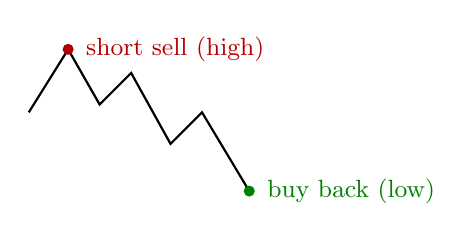
\begin{tikzpicture}
    \draw[thick] (0,0) -- (0.5,0.8) -- (0.9,0.1) -- (1.3,0.5) -- (1.8,-0.4) -- (2.2,0) -- (2.8,-1.0);
    \fill[red!70!black] (0.5,0.8) circle (2pt) node[right=3pt] {\small short sell (high)};
    \fill[green!50!black] (2.8,-1.0) circle (2pt) node[right=3pt] {\small buy back (low)};
\end{tikzpicture}
\end{center}

\b{Terminology}:
\begin{itemize}
    \item \b{Long}: hold a positive position in an asset (buy). \b{Short}: hold a negative position (sell before you buy).
    \item \b{Bull market}: market going up. \b{Bear market}: market going down.
\end{itemize}
Quick fact: for the stock market as a whole, $\overline{r} \approx 11\%$ and $\sigma_r \approx 15\%$.

\header{Diversification}
Why form portfolios? \ul{Portfolios can reduce risk (variance) without sacrificing mean return.}

Consider $n$ \dbb{independent} assets with the same mean and variance, $(\overline{r}_i, \sigma_i^2) = (\overline{r}, \sigma^2)$, and weights $w_1 = \cdots = w_n = \frac{1}{n}$:
\[\overline{r}_p = \sum_{i=1}^{n}w_i\overline{r}_i = \sum_{i=1}^{n}\frac{1}{n}\overline{r} = \overline{r} \qquad \sigma_p^2 = \sum_{i=1}^{n}w_i^2\sigma_i^2 = \sum_{i=1}^{n}\frac{1}{n^2}\sigma^2 = \boxed{\frac{\sigma^2}{n}}\]
\keypoint{Variance is reduced by a factor of $n$, with the same mean. \rb{Portfolios reduce risk!!}}

\begin{example}[Correlated Assets]
    If instead each pair has correlation $\rho$ (here $\sigma^2 = 1$, $\rho = 0.5$), the equal-weight variance is
    \[\sigma_p^2 = \frac{\sigma^2}{n} + \left(1 - \frac{1}{n}\right)\rho\sigma^2 \;\longrightarrow\; \rho\sigma^2 = 0.5 \quad \text{as } n \to \infty\]
    \begin{center}
    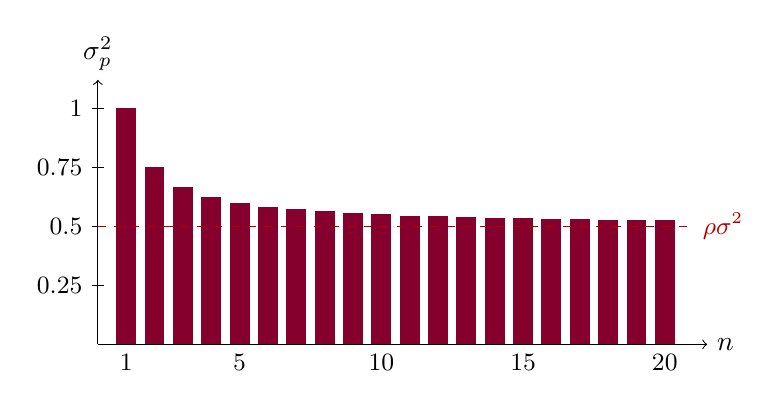
\begin{tikzpicture}[x=0.36cm, y=3cm]
        \draw[->] (0,0) -- (21.5,0) node[right] {$n$};
        \draw[->] (0,0) -- (0,1.12) node[above] {$\sigma_p^2$};
        \foreach \y in {0.25,0.5,0.75,1} { \draw (0.2,\y) -- (-0.2,\y) node[left] {\small \y}; }
        \foreach \n in {1,...,20} {
            \pgfmathsetmacro{\v}{1/\n + 0.5*(1 - 1/\n)}
            \fill[purple!70!black] (\n-0.35,0) rectangle (\n+0.35,\v);
        }
        \foreach \n in {1,5,10,15,20} { \node[below] at (\n,0) {\small \n}; }
        \draw[dashed, red!70!black] (0,0.5) -- (21,0.5) node[right] {\small $\rho\sigma^2$};
    \end{tikzpicture}
    \end{center}
    Diversification removes the independent part of the risk, but not the correlated part: the variance levels off at $0.5$, not $0$.
\end{example}

\header{Portfolio Diagrams}
\heading{Mean-Standard Deviation Diagrams}
Plot each asset or portfolio as a point $(\sigma, \overline{r})$. Where does a portfolio of two assets lie? With $w_1 = \alpha$ and $w_2 = 1 - \alpha$:
\[\boxed{\begin{aligned}
    \text{mean return:} &\quad \overline{r}_p = \alpha\overline{r}_1 + (1-\alpha)\overline{r}_2\\
    \text{variance:} &\quad \sigma_p^2 = \alpha^2\sigma_1^2 + 2\alpha(1-\alpha)\sigma_{12} + (1-\alpha)^2\sigma_2^2\\
    \text{standard deviation:} &\quad \sigma_p = \sqrt{\alpha^2\sigma_1^2 + 2\alpha(1-\alpha)\rho\sigma_1\sigma_2 + (1-\alpha)^2\sigma_2^2}
\end{aligned}}\]

As $\alpha$ goes from 1 to 0, the portfolio traces a curve from asset 1 to asset 2. The curve's shape depends on $\rho$:
\begin{center}
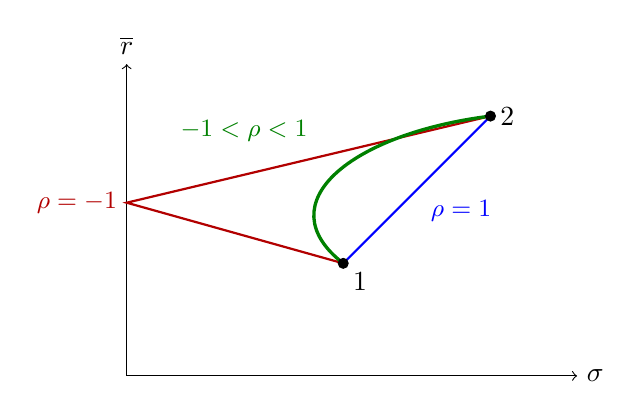
\begin{tikzpicture}[x=1.1cm, y=1.1cm]
    \draw[->] (0,0) -- (5.2,0) node[right] {$\sigma$};
    \draw[->] (0,0) -- (0,3.6) node[above] {$\overline{r}$};
    \coordinate (A) at (2.5,1.3);
    \coordinate (B) at (4.2,3.0);
    % rho = 1: straight line
    \draw[thick, blue] (A) -- (B);
    % rho = -1: through the vertical axis
    \draw[thick, red!70!black] (A) -- (0,2.0) -- (B);
    % 0 < rho < 1: bowed curve
    \draw[very thick, green!50!black] (A) .. controls (1.6,2.0) and (2.6,2.8) .. (B);
    \fill (A) circle (2pt) node[below right] {1};
    \fill (B) circle (2pt) node[right] {2};
    \node[blue, right] at (3.4,1.9) {\small $\rho = 1$};
    \node[red!70!black, left] at (0,2.0) {\small $\rho = -1$};
    \node[green!50!black, above left] at (2.2,2.6) {\small $-1 < \rho < 1$};
\end{tikzpicture}
\end{center}
With $\rho = 1$ the portfolio lies on the straight line between the assets. With $\rho = -1$ there is a portfolio with zero risk. In between, the curve bows to the \ul{left} of the line, which is diversification: less risk for the same mean.

\begin{example}[Mean-Variance Diagram]
    Security 1: $\sigma_1 = 20\%$, $\overline{r}_1 = 8\%$. Security 2: $\sigma_2 = 25\%$, $\overline{r}_2 = 20\%$. Correlation $\rho = 0.5$.
    \begin{center}
    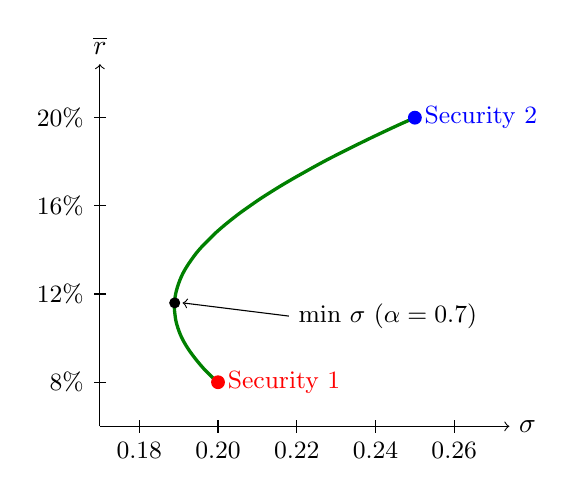
\begin{tikzpicture}
        % sigma -> (sigma-0.17)*50 cm, mean -> (mean-0.06)*28 cm
        \draw[->] (0,0) -- (5.2,0) node[right] {$\sigma$};
        \draw[->] (0,0) -- (0,4.6) node[above] {$\overline{r}$};
        \foreach \x in {0.18,0.20,0.22,0.24,0.26} { \draw ({(\x-0.17)*50},0.08) -- ({(\x-0.17)*50},-0.08) node[below] {\small \x}; }
        \foreach \y/\l in {0.08/8\%,0.12/12\%,0.16/16\%,0.20/20\%} { \draw (0.08,{(\y-0.06)*28}) -- (-0.08,{(\y-0.06)*28}) node[left] {\small \l}; }
        \draw[very thick, green!50!black, domain=0:1, samples=40, smooth, variable=\a]
            plot ({(sqrt(\a*\a*0.04 + 2*\a*(1-\a)*0.5*0.2*0.25 + (1-\a)*(1-\a)*0.0625)-0.17)*50}, {(0.08*\a + 0.20*(1-\a)-0.06)*28});
        \fill[red] ({(0.20-0.17)*50},{(0.08-0.06)*28}) circle (2.5pt) node[right] {\small Security 1};
        \fill[blue] ({(0.25-0.17)*50},{(0.20-0.06)*28}) circle (2.5pt) node[right] {\small Security 2};
        \fill ({(0.189-0.17)*50},{(0.116-0.06)*28}) circle (2pt);
        \draw[<-] ({(0.189-0.17)*50+0.1},{(0.116-0.06)*28}) -- (2.4,1.4) node[right] {\small min $\sigma$ ($\alpha = 0.7$)};
    \end{tikzpicture}
    \end{center}
    E.g.\ $\alpha = 0.5$: $\overline{r}_p = 14\%$, $\sigma_p = \sqrt{0.25(0.04) + 2(0.25)(0.5)(0.2)(0.25) + 0.25(0.0625)} = 0.195$. The smallest risk, $\sigma_p \approx 0.189$, is at $\alpha \approx 0.7$, which is \dbb{below either security's own risk}.
\end{example}

\heading{The Feasible Set}
Given $n$ assets, what does the set of all possible portfolios look like in $(\sigma, \overline{r})$ space?
\begin{itemize}
    \item \b{Without shorting}: a bounded region, with a bullet-shaped left edge and a scalloped right edge.
    \item \b{With shorting}: a larger region. Its left edge is a full hyperbola-like curve that extends without bound.
\end{itemize}
\begin{center}
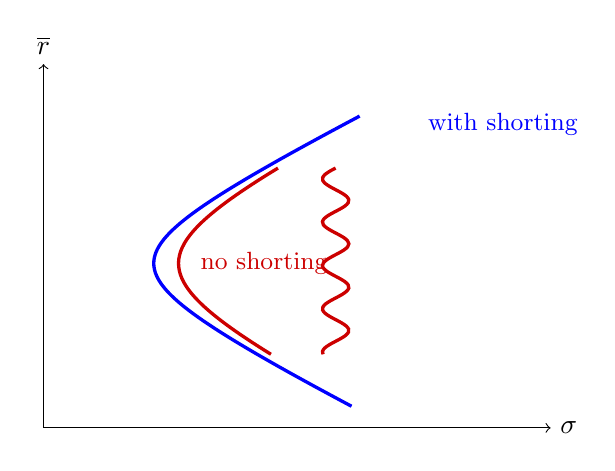
\begin{tikzpicture}[x=1.4cm, y=1.1cm]
    \draw[->] (0,0) -- (4.6,0) node[right] {$\sigma$};
    \draw[->] (0,0) -- (0,4.2) node[above] {$\overline{r}$};
    % with shorting: min-variance set
    \draw[very thick, blue, domain=0.25:3.6, samples=60, smooth, variable=\r] plot ({sqrt(1 + 2.5*(\r-1.9)^2)}, {\r});
    % without shorting: bullet with wavy right edge
    \draw[very thick, red!80!black, domain=0.85:3.0, samples=50, smooth, variable=\r] plot ({sqrt(1.5 + 2.5*(\r-1.9)^2)}, {\r});
    \draw[very thick, red!80!black, domain=0.85:3.0, samples=60, smooth, variable=\r] plot ({2.65 + 0.12*sin(\r*720)}, {\r});
    \node[red!80!black] at (2.0,1.9) {\small no shorting};
    \node[blue, right] at (3.4,3.5) {\small with shorting};
\end{tikzpicture}
\end{center}
The slide's spreadsheet example (three uncorrelated assets with means 9\%, 15\%, 20\%, no shorting) shows the feasible points filling a bullet-shaped region to the left of the individual assets.

\heading{The Minimum Variance Set and Efficient Frontier}
If you are \dbb{risk averse}:
\begin{itemize}
    \item For a given mean return, you minimize the variance (risk). So your portfolio is always on the \rb{minimum-variance set}: the left boundary of the feasible region.
    \item For a given variance (risk level), you maximize your mean return. So you only want the \ul{top portion} of the minimum-variance set: the \rb{efficient frontier}.
\end{itemize}
\begin{center}
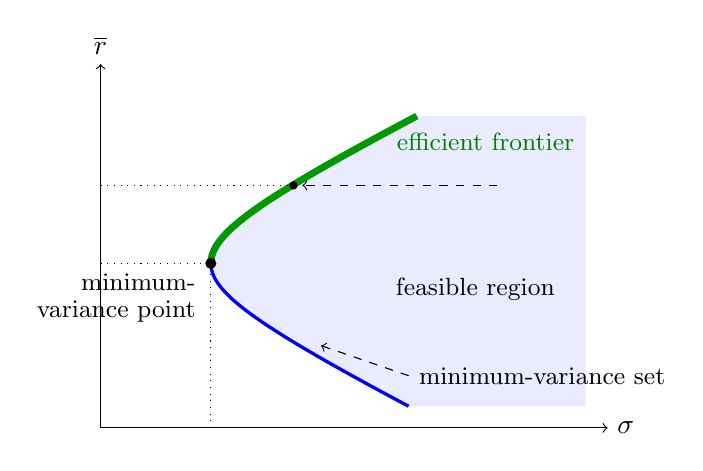
\begin{tikzpicture}[x=1.4cm, y=1.1cm]
    \fill[blue!8, domain=0.25:3.6, samples=60, smooth, variable=\r] plot ({sqrt(1 + 2.5*(\r-1.9)^2)}, {\r}) -- (4.4,3.6) -- (4.4,0.25) -- cycle;
    \draw[->] (0,0) -- (4.6,0) node[right] {$\sigma$};
    \draw[->] (0,0) -- (0,4.2) node[above] {$\overline{r}$};
    \draw[very thick, blue, domain=0.25:3.6, samples=60, smooth, variable=\r] plot ({sqrt(1 + 2.5*(\r-1.9)^2)}, {\r});
    \draw[line width=2.5pt, green!60!black, domain=1.9:3.6, samples=40, smooth, variable=\r] plot ({sqrt(1 + 2.5*(\r-1.9)^2)}, {\r});
    \draw[dotted] (0,1.9) -- (1,1.9);
    \draw[dotted] (1,0) -- (1,1.9);
    \fill (1,1.9) circle (2pt);
    \node[left, align=right] at (0.95,1.5) {\small minimum-\\[-2pt]\small variance point};
    \node[green!50!black, right] at (2.6,3.3) {\small efficient frontier};
    \node at (3.4,1.6) {\small feasible region};
    \draw[<-, dashed] (2.0,0.95) -- (2.8,0.6) node[right] {\small minimum-variance set};
    % arrow: min variance point for a given mean
    \draw[dotted] (0,2.8) -- (1.8,2.8);
    \draw[->, dashed] (3.6,2.8) -- (1.83,2.8);
    \fill (1.75,2.8) circle (1.5pt);
\end{tikzpicture}
\end{center}
The horizontal dashed arrow: at a fixed mean return, move left (less risk) until you hit the minimum-variance set.

\header{Linear Algebra Formulation}
\heading{Linear Algebra Basics}
For $x, y \in \R^n$ and $A \in \R^{n\times n}$:
\[x^Ty = \sum_{i=1}^{n}x_iy_i \qquad Ax = \begin{bmatrix}\sum_{i}a_{1i}x_i\\ \vdots\\ \sum_{i}a_{ni}x_i\end{bmatrix} \qquad x^TAy = \sum_{j=1}^{n}\sum_{i=1}^{n}a_{ji}x_jy_i\]
Matrix multiplication does \dbb{not commute}: $AB \neq BA$ in general. Transpose and inverse reverse the order:
\[(AB)^T = B^TA^T \qquad (AB)^{-1} = B^{-1}A^{-1}\]

\heading{Random Vectors}
For a random vector $X = (X_1, \dots, X_n)^T$:
\[\overline{X} = E[X] = \begin{bmatrix}\overline{X}_1\\ \vdots\\ \overline{X}_n\end{bmatrix} \qquad \Sigma = E\left[(X - \overline{X})(X - \overline{X})^T\right] = \begin{bmatrix}\sigma_{11} & \sigma_{12} & \cdots & \sigma_{1n}\\ \sigma_{21} & \sigma_{22} & \cdots & \sigma_{2n}\\ \vdots & & \ddots & \vdots\\ \sigma_{n1} & \sigma_{n2} & \cdots & \sigma_{nn}\end{bmatrix}\]
$\Sigma$ is the \rb{covariance matrix}: symmetric, with the variances on the diagonal.

Let $Y = a^TX$. Then
\begin{align*}
    \overline{Y} &= E[a^TX] = a^TE[X] = a^T\overline{X}\\
    \sigma_Y^2 = \operatorname{Var}(a^TX) &= E\left[\left(a^T(X - \overline{X})\right)^2\right] = E\left[a^T(X - \overline{X})(X - \overline{X})^Ta\right]\\
    &= a^TE\left[(X - \overline{X})(X - \overline{X})^T\right]a = a^T\Sigma a
\end{align*}

\heading{Linear Algebra and Returns}
With $w = (w_1, \dots, w_n)^T$, $r = (r_1, \dots, r_n)^T$, $\overline{r} = (\overline{r}_1, \dots, \overline{r}_n)^T$ and covariance matrix $\Sigma = E[(r - \overline{r})(r - \overline{r})^T]$:
\[\boxed{r_p = w^Tr \qquad \overline{r}_p = w^T\overline{r} \qquad \sigma_p^2 = w^T\Sigma w}\]

\begin{example}[Using Linear Algebra]
    The two-asset example again:
    \[w = \begin{bmatrix}0.25\\ 0.75\end{bmatrix} \qquad \overline{r} = \begin{bmatrix}0.12\\ 0.15\end{bmatrix} \qquad \Sigma = \begin{bmatrix}(0.20)^2 & 0.01\\ 0.01 & (0.18)^2\end{bmatrix}\]
    \[\overline{r}_p = w^T\overline{r} = 0.1425 \qquad \sigma_p^2 = w^T\Sigma w = 0.0245\]
    Same answers as before, but this form scales to any number of assets.
\end{example}
